\documentclass[a4paper]{article}
\usepackage{graphicx}
\usepackage{geometry}
\usepackage{calc}
\usepackage[percent]{overpic}
\usepackage[medium]{HindMadurai}
\usepackage[T1]{fontenc}
\usepackage{tikz}
\usepackage{multicol}
\usepackage{enumitem}
\usepackage{xcolor}

% \renewcommand\familydefault{\sfdefault}

\newlength{\picmargin}
\setlength{\picmargin}{15pt}

\newlength{\picwidth}
\setlength{\picwidth}{\paperwidth - 2\picmargin}

\geometry{
    top=\picmargin,
    bottom=\picmargin,
    left=\picmargin,
    textwidth=\picwidth
}

\newcommand{\recipeTitle}[1]{
  \vspace{0.2cm}
  \parbox{\picwidth}{
    \centering
    \LARGE{\textbf{#1}}
  }
}

\newcommand{\recipeDescription}[1]{
  \vspace{0.2cm}
  \parbox{\picwidth}{
    \centering
    \large
    {#1}
  }
}

\newcommand{\ingredient}[1]{
  \vspace{0.1cm}
  \hspace{0cm}
  {#1}\\
}

\newcommand{\prep}[1]{
  \textbf{Prep:} {#1}\\
}

\newcommand{\cooking}[1]{
  \textbf{Cook:} {#1}\\
}

\newcommand{\hide}[1]
{}

\definecolor{Pagebackground}{HTML}
{eeeeee} %<{type: "reference", id: "backgroundColor"}>
\pagecolor{Pagebackground}

\definecolor{captionColor}{HTML}
{000000} %<{type: "reference", id: "imageCaptionColor"}>

\definecolor{textColor}{HTML}
{000000} %<{type: "reference", id: "textColor"}>

\begin{document}
\pagestyle{empty}
%<{"type": "group", "description": "Recipe image"}
\hspace{-\picmargin}%
\begin{overpic}[
    width=\picwidth,
    height=0.70\picwidth,
    % grid,
    % tics=10
  ]
  %<{
  %   type: "crop",
  %   description: "",
  %   aspect: 1.43,
  %   inputValue: "raspberry-pie-cropped"
  % }>
    {raspberry-pie-cropped}
  %>
  \put (1,2) {
    \parbox[b]{0.3\picwidth}
    {
      \textcolor{captionColor}{
        \textbf
        %<{
        %   type: "text",
        %   description: "Recipe image caption",
        %   inputValue: "Caption. Say something sweet about this photo or recipe."
        % }>
          {Caption. Say something sweet about this photo or recipe.}
        %>
      }
    }
  }
\end{overpic}
%>

\color{textColor}

\vspace{0.5cm}
\hspace{-\picmargin}
%<{
%   type: "text",
%   description: "Recipe title",
%   inputValue: "NANA'S RASPBERRY PIE"
% }>
\recipeTitle{NANA'S RASPBERRY PIE}
%>

\vspace{-0.5cm}
\hspace{-\picmargin}
\parbox{\picwidth}{
  \centering
  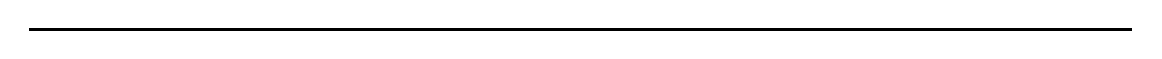
\begin{tikzpicture}
    \draw[very thick] (-7,0) -- (7,0);
  \end{tikzpicture}
}
% \line(1,0){12cm}

\vspace{0.3cm}
\hspace{-\picmargin}
\recipeDescription{There was nothing like Nana's Raspberry Pie when we were younger. It's sweet, a bit tart, and tastes like summers on the porch in North Carolina.} %<{type: "textblock", description: "Recipe description", injectBrackets: true, inputValue: "There was nothing like Nana's Raspberry Pie when we were younger. It's sweet, a bit tart, and tastes like summers on the porch in North Carolina."}>

\begin{multicols}{3}
  \normalsize
  \raggedright
  \textbf{Ingredients}\\
  \vspace{0.2cm}
  %<{"type": "list", "description": "Ingredients"}
    %<{"type": "text", "description": "Your ingredient", inputValue: "2 cups all-purpose flour"}
      \ingredient{2 cups all-purpose flour}
    %>
    %<{"type": "text", "description": "Your ingredient", inputValue: "1.5 teaspoons unsweetened cocoa"}
      \ingredient{1.5 teaspoons unsweetened cocoa}
    %>
    %<{"type": "text", "description": "Your ingredient", inputValue: "1 cup butter (do not user margarine)"}
      \ingredient{1 cup butter (do not user margarine)}
    %>
    %<{"type": "text", "description": "Your ingredient", inputValue: "2 large eggs"}
      \ingredient{2 large eggs}
    %>
    %<{"type": "text", "description": "Your ingredient", inputValue: "0.75 cups sugar"}
      \ingredient{0.75 cups sugar}
    %>
    %<{"type": "text", "description": "Your ingredient", inputValue: "0.25 tablespoons pure vanilla extract"}
      \ingredient{0.25 tablespoons pure vanilla extract}
    %>
  %>
  %<{"type": "group", "description": "Preparation time"}
    \vspace{0.5cm}
    \prep{45 min} %<{"type": "text", "description": "Preparation time", inputValue: "45 min"}>
    \cooking{1.5 hours} %<{"type": "text", "description": "Cooking time", inputValue: "1.5 hours"}>
  %>
  \columnbreak
  \begin{enumerate}[leftmargin=0.3cm]
    %<{"type": "list", "description": "Preparation and cooking steps"}
    \item{Morbi in sem quis dui placerat ornare. Pellentesque odio nisi, euismod in, pharetra a, ultricies in, diam. Sed arcu. Cras consequat} %<{type: "textblock", description: "Your recipe step", injectBrackets: true, inputValue: "Morbi in sem quis dui placerat ornare. Pellentesque odio nisi, euismod in, pharetra a, ultricies in, diam. Sed arcu. Cras consequat"}>
    \item{Praesent dapibus, neque id cursus faucibus, tortor neque egestas augue, eu vulputate magna eros eu erat. Aliquam erat volutpat. Nam dui mi, tincidunt quis, accumsan porttitor, facilisis luctus, metus.} %<{type: "textblock", description: "Your recipe step", injectBrackets: true, inputValue: "Praesent dapibus, neque id cursus faucibus, tortor neque egestas augue, eu vulputate magna eros eu erat. Aliquam erat volutpat. Nam dui mi, tincidunt quis, accumsan porttitor, facilisis luctus, metus."}>
    \item{Phasellus ultrices nulla quis nibh. Quisque a lectus. Donec consectetuer ligula vulputate sem tristique cursus. Nam nulla quam, gravida non, commodo a, sodales sit amet, nisi.} %<{type: "textblock", description: "Your recipe step", injectBrackets: true, inputValue: "Phasellus ultrices nulla quis nibh. Quisque a lectus. Donec consectetuer ligula vulputate sem tristique cursus. Nam nulla quam, gravida non, commodo a, sodales sit amet, nisi."}>
    \item{Pellentesque fermentum dolor. Aliquam quam lectus, facilisis auctor, ultrices ut, elementum vulputate, nunc.} %<{type: "textblock", description: "Your recipe step", injectBrackets: true, inputValue: "Pellentesque fermentum dolor. Aliquam quam lectus, facilisis auctor, ultrices ut, elementum vulputate, nunc."}>
    \item{Sed adipiscing ornare risus. Morbi est est, blandit sit amet, sagittis vel, euismod vel, velit. Pellentesque egestas sem. Suspendisse commodo ullamcorper magna.} %<{type: "textblock", description: "Your recipe step", injectBrackets: true, inputValue: "Sed adipiscing ornare risus. Morbi est est, blandit sit amet, sagittis vel, euismod vel, velit. Pellentesque egestas sem. Suspendisse commodo ullamcorper magna."}>
    \item{Nulla sed leo. Class aptent taciti sociosqu ad litora torquent per conubia nostra, per inceptos himenaeos.
          Fusce lacinia arcu et nulla. Nulla vitae mauris non felis mollis faucibus.} %<{type: "textblock", description: "Your recipe step", injectBrackets: true, inputValue: "Nulla sed leo. Class aptent taciti sociosqu ad litora torquent per conubia nostra, per inceptos himenaeos. Fusce lacinia arcu et nulla. Nulla vitae mauris non felis mollis faucibus."}>
    \item{Lorem ipsum dolor sit amet, consectetuer adipiscing elit. Donec odio. Quisque volutpat mattis eros. Nullam malesuada erat ut turpis. Suspendisse urna nibh, viverra non, semper suscipit, posuere a, pede.} %<{type: "textblock", description: "Your recipe step", injectBrackets: true, inputValue: "Lorem ipsum dolor sit amet, consectetuer adipiscing elit. Donec odio. Quisque volutpat mattis eros. Nullam malesuada erat ut turpis. Suspendisse urna nibh, viverra non, semper suscipit, posuere a, pede."}>
    \item{Donec nec justo eget felis facilisis fermentum. Aliquam porttitor mauris sit amet orci. Aenean dignissim pellentesque felis.} %<{type: "textblock", description: "Your recipe step", injectBrackets: true, inputValue: "Donec nec justo eget felis facilisis fermentum. Aliquam porttitor mauris sit amet orci. Aenean dignissim pellentesque felis."}>
    \item{Morbi in sem quis dui placerat ornare. Pellentesque odio nisi, euismod in, pharetra a, ultricies in, diam. Sed arcu. Cras consequat.} %<{type: "textblock", description: "Your recipe step", injectBrackets: true, inputValue: "Morbi in sem quis dui placerat ornare. Pellentesque odio nisi, euismod in, pharetra a, ultricies in, diam. Sed arcu. Cras consequat."}>
    %>
  \end{enumerate}
\end{multicols}

%<{type: "group", description: "Color settings (optional)"}
\hide{
  %<{type: "color", description: "Page background color", initialColor: "#EEEEEE", id: "backgroundColor", inputValue: "EEEEEE"}>
  %<{type: "color", description: "Image caption color", initialColor: "#000000", id: "imageCaptionColor", inputValue: "000000"}>
  %<{type: "color", description: "Text color", initialColor: "#000000", id: "textColor", inputValue: "000000"}>
}
%>

\end{document}